% =============================================================================
%  §III.2.2 — Critère C60 : la récursion transfinie VÉRITABLE (chantier R')
%  Fragment du rapport V9 (style : frag_iii6_denombrable.tex).
%  Code : bourbaki/iii_.../iii_2_bien_ordonnes/bon_ordre/recurrence_transfinie/
%         rec_veritable/ (+ sous-dossier couverture_rec/).
% =============================================================================

\subsection{§III.2.2, Critère C60 --- la récursion transfinie \emph{véritable} (chantier R$'$)}

\textbf{Énoncé (Bourbaki, E III.18--19).} « Soient $u$ une lettre, $\mathrm{T}\{u\}$
un terme de la théorie $\mT$. Il existe un ensemble $\mathrm{U}$ et une application
$f$ de $E$ sur $\mathrm{U}$ tels que, pour tout $x \in E$, on ait
$f(x) = \mathrm{T}\{f^{(x)}\}$. En outre, l'ensemble $\mathrm{U}$ et l'application
$f$ sont déterminés de façon unique par ces conditions. » Ici $E$ est bien ordonné
et $f^{(x)}$ désigne l'application qui coïncide avec $f$ sur le segment ouvert
$\seg_x = {]\!\leftarrow, x[}$ --- c'est-à-dire \emph{la restriction} $f|\seg_x$.
L'équation de récursion lit donc le \emph{passé entier} de $f$ sous $x$, pas le
seul point $x$.

\textbf{Pourquoi le chantier (l'écart comblé).} La version antérieure du dépôt
(chantier C60/C62 « hygienic ») certifiait l'existence d'une fonction $f$
vérifiant $f(z) = h(z)$ --- la règle $h : \text{Terme}\to\text{Terme}$ appliquée
\emph{au point} $z$, jamais à $f$ : une \emph{tabulation} (le graphe de $h$),
écart de fidélité avoué de \texttt{fonction\_existence} et consigné au journal
(2026-08-22). Une clef-raccourci (réinjecter $h(z) := \mathrm{T}\{f|\seg_z\}$
dans le capstone déposé) a été \emph{rejetée pour soundness} : l'axiome de
sélection S8 de la famille mentionnerait alors le terme qu'il définit --- un
point fixe imprédicatif, hors du schéma S8. D'où la refonte R$'$ : re-dériver
essai, unicité, prolongement, descente et famille avec la vraie équation
$p(z) = \mathrm{T}\{p|\seg_z\}$, la règle restant un callable \emph{opaque}
\texttt{vh} (aucun axiome sur elle). \\
Modules : \texttt{recurrence\_transfinie/rec\_veritable/} (six fichiers) et
\texttt{rec\_veritable/couverture\_rec/} (sept fichiers). Dans toute la suite,
$D_x := \seg_x \cup \{x\}$ (le « domaine d'essai », \texttt{dom\_essai}) et
\emph{bo} abrège $\mathrm{est\_bien\_ordonne}(R, E)$.

\subsection{C60-R1$'$ --- le prédicat d'essai récursif (l'équation lit la restriction)}
\textbf{Formalisé} (\texttt{rec\_veritable/ensembles\_essai\_rec.py}) :
\[
  \mathrm{est\_essai\_rec}(p, \mathrm{T}, x) \;:=\;
  \mathrm{func}(p) \;\wedge\; \mathrm{dom}\,p = D_x \;\wedge\;
  (\forall z)\bigl(z \in \mathrm{dom}\,p \Rightarrow
    p(z) = \mathrm{T}\{\,p|\seg_z\,\}\bigr).
\]
C'est le prédicat d'essai de la démonstration de C60 avec la \emph{vraie}
équation : $\mathrm{T}$ reçoit la restriction $p|\seg_z$, et l'équation vaut sur
\emph{tout} le domaine. Le lieur du $\forall$ est un nom frais (\texttt{zesr}) :
la règle peut lier en interne ses propres variables ($\tau$-cardinaux), et
quantifier sur un nom qu'elle lie capturerait à la construction (leçon des
liants exotiques du capstone C62). \textbf{Statut.} Définition (formule pure) :
aucun axiome, aucun théorème, \texttt{theorie\_ensembles()==22}.

\subsection{C60-R2$'$ --- unicité : deux essais récursifs au même point sont le même graphe}
\textbf{Formalisé} (\texttt{ensembles\_unicite\_essai\_rec.py}, cible
\texttt{unicite\_essai\_rec}) :
\[
  \{\,\text{bo},\ \mathrm{est\_essai\_rec}(p, x),\ \mathrm{est\_essai\_rec}(q, x),\
     x \in E,\ \mathrm{graphe}(p),\ \mathrm{graphe}(q)\,\} \;\vdash\; p = q
\]
(six hypothèses honnêtes).
\textbf{Preuve (\Nstar).} Quatre briques posent l'égalité des restrictions
(\texttt{restrictions\_egales}, 7 hyp.) : seg-transitivité stricte
$\{$bo$\} \vdash (z \in \seg_x \wedge u \in \seg_z) \Rightarrow u \in \seg_x$
(transitivité + antisymétrie extraites du bon ordre), donc
$\seg_z \subset D_x = \mathrm{dom}\,p$ ; les deux restrictions $p|\seg_z$ et
$q|\seg_z$ ont alors le même domaine $\seg_z$ et, sous l'hypothèse de récurrence
transfinie, les mêmes valeurs --- l'extensionnalité fonctionnelle
(\texttt{graphe\_egal\_par\_valeurs}, 6 prémisses) conclut. Le pas
(\texttt{unicite\_au\_point}, 5 hyp.) transporte cette égalité \emph{à travers la
règle opaque} par la congruence C44 : $p(z) = \mathrm{T}\{p|\seg_z\} =
\mathrm{T}\{q|\seg_z\} = q(z)$. L'induction C59 referme : le prédicat est
\emph{gardé par le domaine}, $\mathrm{couvert}[t] := (t \in D_x \Rightarrow
p(t) = q(t))$ --- hors de $D_x$ les valeurs sont du bruit-$\tau$ et la garde rend
l'hérédité prouvable ; le dégardage point par point passe par
$\seg_z \subset D_x$. Enfin $D_x \subset E$ (sous $x \in E$) ramène la
couverture sur tout $\mathrm{dom}\,p$ et l'extensionnalité donne $p = q$.
\textbf{Statut.} CLOS sous les 6 hypothèses honnêtes (séquent exact, aucune
parasite) ; 6 ticks d'écriture, 9 tests.

\subsection{C60-R3$'$ --- le prolongement d'un pas : $p' := p \cup \{(x, \mathrm{T}\{p\})\}$}
\textbf{Formalisé} (\texttt{ensembles\_extension\_essai.py} +
\texttt{ensembles\_extension\_assemblage.py}, cible \texttt{extension\_essai\_rec}) :
\[
  \{\,\text{bo},\ \mathrm{func}(p),\ \mathrm{dom}\,p = \seg_x,\
     \mathrm{graphe}(p),\ \text{éq-seg}(p)\,\} \;\vdash\;
  \mathrm{est\_essai\_rec}\bigl(p \cup \{(x, \mathrm{T}\{p\})\},\ x\bigr)
\]
(cinq hypothèses honnêtes), où éq-seg$(p)$ est l'équation-restriction sur
$\mathrm{dom}\,p$ (la forme \texttt{equation\_sur\_seg}). \textbf{Preuve (\Nstar).} La clé conceptuelle : la
valeur au nouveau point est $\mathrm{T}\{p\}$ --- la règle appliquée à $p$
\emph{entier}, qui est exactement $p'|\seg_x$. Trois briques : la restriction
\emph{efface} le nouveau point, $\{\neg(x \in X)\} \vdash (p \cup \{(x,v)\})|X
= p|X$ (double inclusion par l'axiome-restriction, cas singleton absurde) ;
$\vdash \neg(x \in \seg_x)$ [CLOS] ; la restriction pleine
$\{\mathrm{graphe}(p)\} \vdash p|\mathrm{dom}\,p = p$. L'équation de $p'$ se
vérifie par cas : en $z \in \seg_x$, $p'(z) = p(z) = \mathrm{T}\{p|\seg_z\} =
\mathrm{T}\{p'|\seg_z\}$ ($x \notin \seg_z$ par seg-transitivité, sinon
$x \in \seg_x$ ; congruence C44) ; en $z = x$, $p'(x) = \mathrm{T}\{p\}$ et
$p'|\seg_x = p|\seg_x = p$ (effacement + restriction pleine), congruence puis
réécriture $z \to x$. \textbf{Statut.} CLOS sous les 5 hypothèses honnêtes ;
le pas tient en $\sim$90 lignes grâce à la carte de réutilisation
(\texttt{extension\_un\_pas\_fonctionnelle}, \texttt{valeur\_reunion\_*},
domaines binaires du C60 déposé).

\subsection{C60-R4$'$ --- la descente : restreindre un essai reste un essai}
\textbf{Formalisé} (\texttt{couverture\_rec/ensembles\_composition\_restrictions.py}
et \texttt{ensembles\_restriction\_essai.py}) :
\[
  \{\,B \subset A\,\} \vdash (p|A)|B = p|B \qquad \text{[1 hyp.\ honnête]},
\]
\[
  \{\,\text{bo},\ \mathrm{est\_essai\_rec}(p, x),\ y \in D_x\,\} \vdash
  \mathrm{est\_essai\_rec}(p|D_y,\ y) \qquad \text{[3 hyp.\ honnêtes]}.
\]
\textbf{Preuve (\Nstar).} La composition des restrictions (R4$'$b) est une double
inclusion sur l'axiome-restriction, témoins aux liants de l'axiome. La descente
(R4$'$a) : $D_y \subset D_x = \mathrm{dom}\,p$ (monotonie de $D$, 2 hyp.), donc
$p|D_y$ est fonctionnelle de domaine $D_y$ ; son équation en $z$ lit
$(p|D_y)|\seg_z$, qui est $p|\seg_z$ par R4$'$b dès que $\seg_z \subset D_y$
(seg-transitivité), et la congruence C44 recolle. \textbf{Statut.} CLOS sous
hypothèses honnêtes (1 et 3), premier coup, 19 tests cumulés au jalon.

\subsection{C60-R5$'$ --- la famille des essais et sa réunion (l'essai-limite)}
\textbf{Formalisé} (\texttt{couverture\_rec/}, cinq modules). (a)
\emph{Coïncidence sans wlog} (\texttt{ensembles\_coincidence\_famille.py}) :
\[
  \{\,\text{bo},\ \mathrm{est\_essai\_rec}(p, y),\ \mathrm{est\_essai\_rec}(q, y'),\
     a \in D_y,\ a \in D_{y'},\ a \in E\,\} \;\vdash\; p(a) = q(a)
\]
(six hypothèses honnêtes).
Aucune trichotomie, aucun wlog : les \emph{deux} essais descendent au point
commun (R4$'$a) --- $p|D_a$ et $q|D_a$ sont des essais récursifs \emph{en} $a$,
donc égaux (R2$'$ appliqué aux termes-restrictions, conjoints graphe clos par
\texttt{restriction\_est\_graphe}) ; les valeurs se transportent par
\texttt{restriction\_valeur} et le lemme clos $a \in D_a$. (b) \emph{La famille
S8} (\texttt{ensembles\_famille\_rec.py}) :
\[
  \mathrm{Dfam\_rec}(G, E, x, V) :=
  \{\, p \in \mathfrak{P}(E \times V) \mid
      (\exists y)\bigl(y \in \seg_x \wedge \mathrm{est\_essai\_rec}(p, y)\bigr) \,\},
\]
sélection S8 dans un contenant existant (aucune auto-référence : le sélecteur
mentionne $p$, jamais le terme défini), théorie dédiée hors des 22 axiomes.
Amélioration sur le patron déposé (leçon \texttt{seg\_ext}) : le terme
\emph{porte le graphe} $G$ --- deux ordres distincts donnent des termes
distincts, donc jamais deux axiomes incompatibles sur un même terme ; la règle
\texttt{vh}, capturée par l'axiome, reste une limite documentée (ne jamais
mélanger deux règles dans une même preuve). (c) \emph{La réunion}
$\bigcup \mathrm{Dfam\_rec}(x)$ (\texttt{ensembles\_union\_rec.py},
\texttt{ensembles\_domaine\_union.py}, \texttt{ensembles\_equation\_union.py}) :
compatibilité $\{\text{bo}\} \vdash \mathrm{famille\_compatible}$ [1 hyp.] (la
tabulation l'avait gratuite par valeurs épinglées ; la vraie récursion l'obtient
par la coïncidence (a)) ; domaine $\{\text{bo}, \text{antécédent}\} \vdash
\mathrm{dom}\bigl(\bigcup D\bigr) = \seg_x$ [2 hyp.], où l'antécédent est la
couverture-ambiante des $y < x$ (l'hypothèse d'induction de la future hérédité) ;
équation $\{\text{bo}, \text{antécédent}\} \vdash
\text{éq-seg}\bigl(\bigcup D\bigr)$ [2 hyp.] --- la forme \emph{exacte} attendue
par R3$'$ : la réunion est un essai-sur-seg, prête au prolongement.
\textbf{Statut.} CLOS sous hypothèses honnêtes, chaque séquent exact ; briques
ambiantes ($\bigcup D \in \mathfrak{P}(E \times V)$, extension ambiante sous
« $\mathrm{T}$ à valeurs dans $V$ », la donnée même de C60) closes en appui.

\subsection{Techniques notables et statut du chantier}
\textbf{Techniques (consignées au journal).}
(1) \emph{Prédicat C59 gardé par le domaine} : l'induction transfinie porte sur
$t \in D_x \Rightarrow p(t) = q(t)$, jamais sur l'égalité nue --- hors du domaine
elle est indémontrable ; le dégardage est un lemme ($\seg_z \subset D_x$).
(2) \emph{Coïncidence sans wlog} : au lieu d'ordonner $y, y'$ (trichotomie,
non close), descente \emph{bilatérale} des deux essais au point commun, puis
unicité en ce point.
(3) \emph{Le terme de famille porte le graphe} : $\mathrm{Dfam\_rec}(G, \ldots)$
inclut $G$ dans le terme S8, éliminant le conflit d'axiomes de la version
déposée.
(4) \emph{Congruence C44 à travers la règle opaque} :
\texttt{congruence\_terme}$(A, B, \mathrm{T}\{w\}, w)$ transporte $A = B$ en
$\mathrm{T}\{A\} = \mathrm{T}\{B\}$ sans rien savoir de $\mathrm{T}$ --- c'est
elle qui fait vivre la récursion avec une règle arbitraire.
(5) \emph{Liants-paramètres disjoints} : les témoins des éliminations $\exists$
portent les liants des axiomes (« p », « q », \texttt{yDr}/\texttt{zDr}
distincts), les paramètres des lemmes des noms dédiés --- zéro capture sur tout
le chantier.

\textbf{Statut global.} R1$'$--R5$'$ \emph{clos} (27 tests
\texttt{rec\_veritable} verts, \texttt{theorie\_ensembles()==22}, noyau intact,
rien postulé sur la règle). Restent, en cours : R6$'$ --- l'hérédité de la
couverture ($\bigcup D$ recollé puis prolongé par R3$'$ donne l'essai en $x$) et
la couverture totale par C59 ; R7$'$ --- le capstone : existence et unicité de
$f$ sur $E$ avec $f(x) = \mathrm{T}\{f|\seg_x\}$, l'énoncé littéral de C60.

\begin{figure}[h]
  \centering
  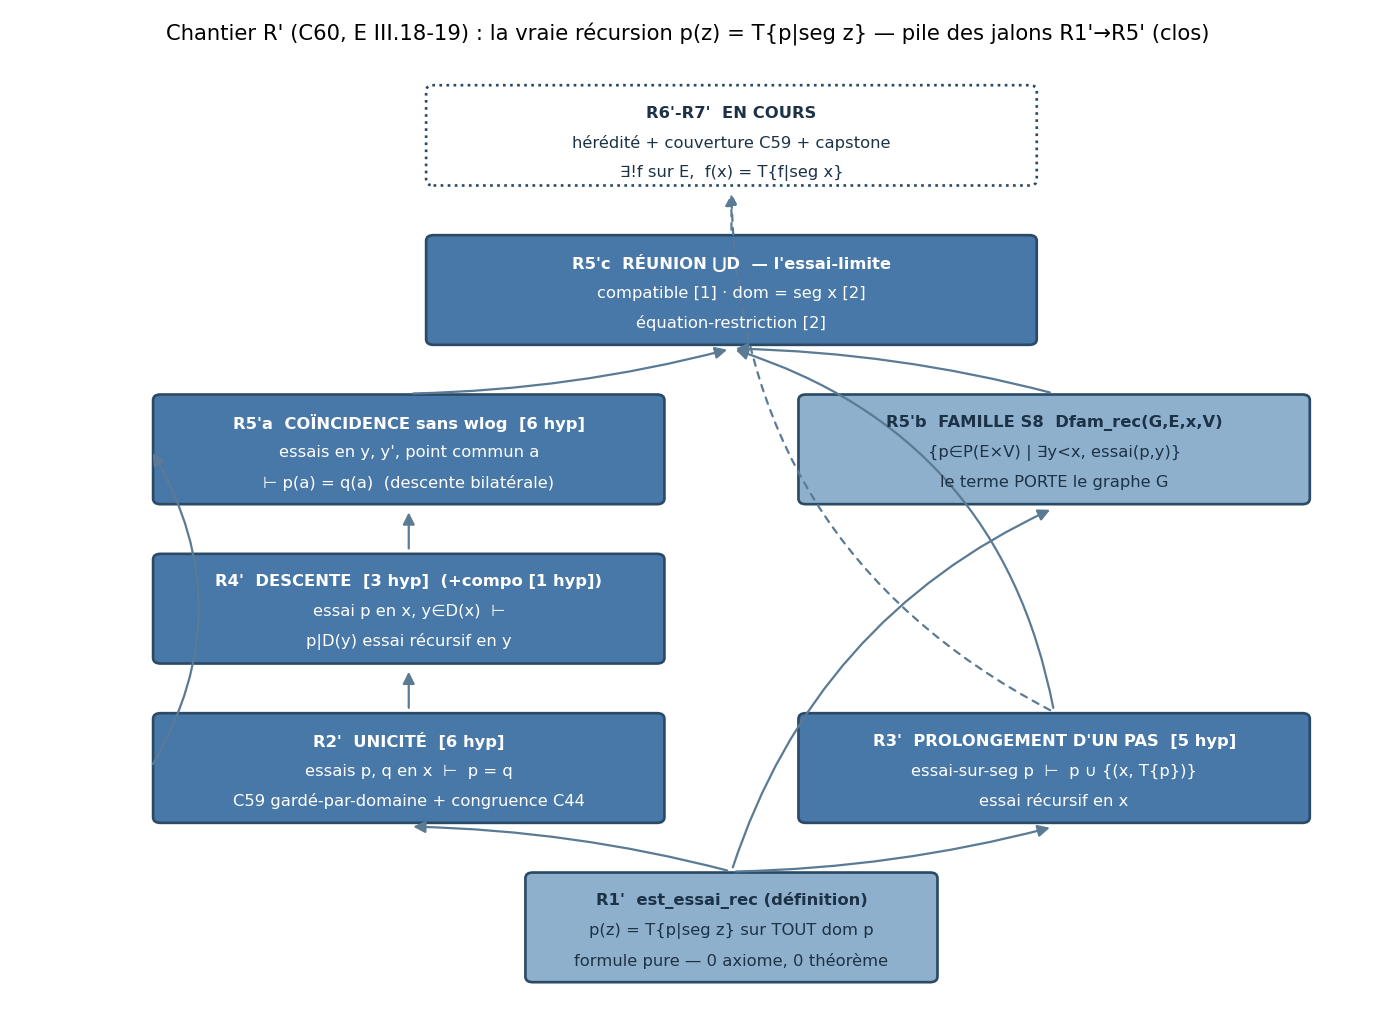
\includegraphics[width=0.92\linewidth]{figures/chantier_recursion.png}
  \caption{La pile de dépendances du chantier R$'$ (récursion transfinie
  véritable, C60) : jalons R1$'$--R5$'$ clos avec leurs séquents (nombre
  d'hypothèses honnêtes entre crochets), flèches = dépendances de preuve ;
  en pointillés, le front R6$'$--R7$'$ (hérédité, couverture C59, capstone).
  Script reproductible \texttt{figures/gen\_chantier\_recursion.py}.}
\end{figure}
